% ============================================================
%  N.2.5  Eyeriss CS2 & CS3: Activation Register Sizing
% ============================================================
\subsection{Eyeriss: Activation Register Sizing (CS2, CS3)}
\label{sec:eyeriss-cs2-cs3}

\subsubsection{Motivation}

Besides the weight register examined in CS1, every PE in the
Eyeriss-Like architecture contains three additional local storage
structures: an \emph{input register} (InReg), which buffers the
first layer's input activations; an \emph{intermediate register}
(IntReg), which buffers the activation values exchanged between
consecutive fused layers; and an \emph{output register} (OutReg),
which holds the final-layer output before it is written back to the
GlobalBuffer.

Of these three, only IntReg (CS2) is genuinely affected by fusion.
The InReg sees exclusively the network's input, regardless of how
many layers are fused: intermediate activations produced inside the
fusion chain never pass through InReg, they are routed to IntReg
instead.
Similarly, the OutReg stores only the last fused layer's output
channel residual, so its footprint does not grow with the number of
fused layers.

We will analyze InReg and OutReg in a unique case study CS3.

Under full fusion the IntReg must accommodate the residual channel
factors of \emph{all} intermediate activations, i.e.\ the $Z_i$
values that the spatial-array columns (SACols) cannot absorb.
The footprint therefore scales with the number of fused layers and
with the width of their channel dimensions.


% ────────────────────────────────────────────────────────────────────
\label{sec:eyeriss-cs2}

\paragraph{CS2 per Weight-dominant workloads (ResNet18, VGG16)}: \\



The table reveals the same doubling rule observed for WReg in CS1.


Figure~\ref{fig:eyeriss-cs2-inv} the horizontal axis is the PE budget and the vertical axis is
the minimum IntReg that makes the fused mapping feasible.
Reading the curve from left to right, one can directly read off the
register size that a given area constraint demands.
The slope is consistent with the doubling rule: every $2\times$
reduction in PE budget roughly doubles the minimum IntReg.

\begin{figure}[htbp]
  \centering
  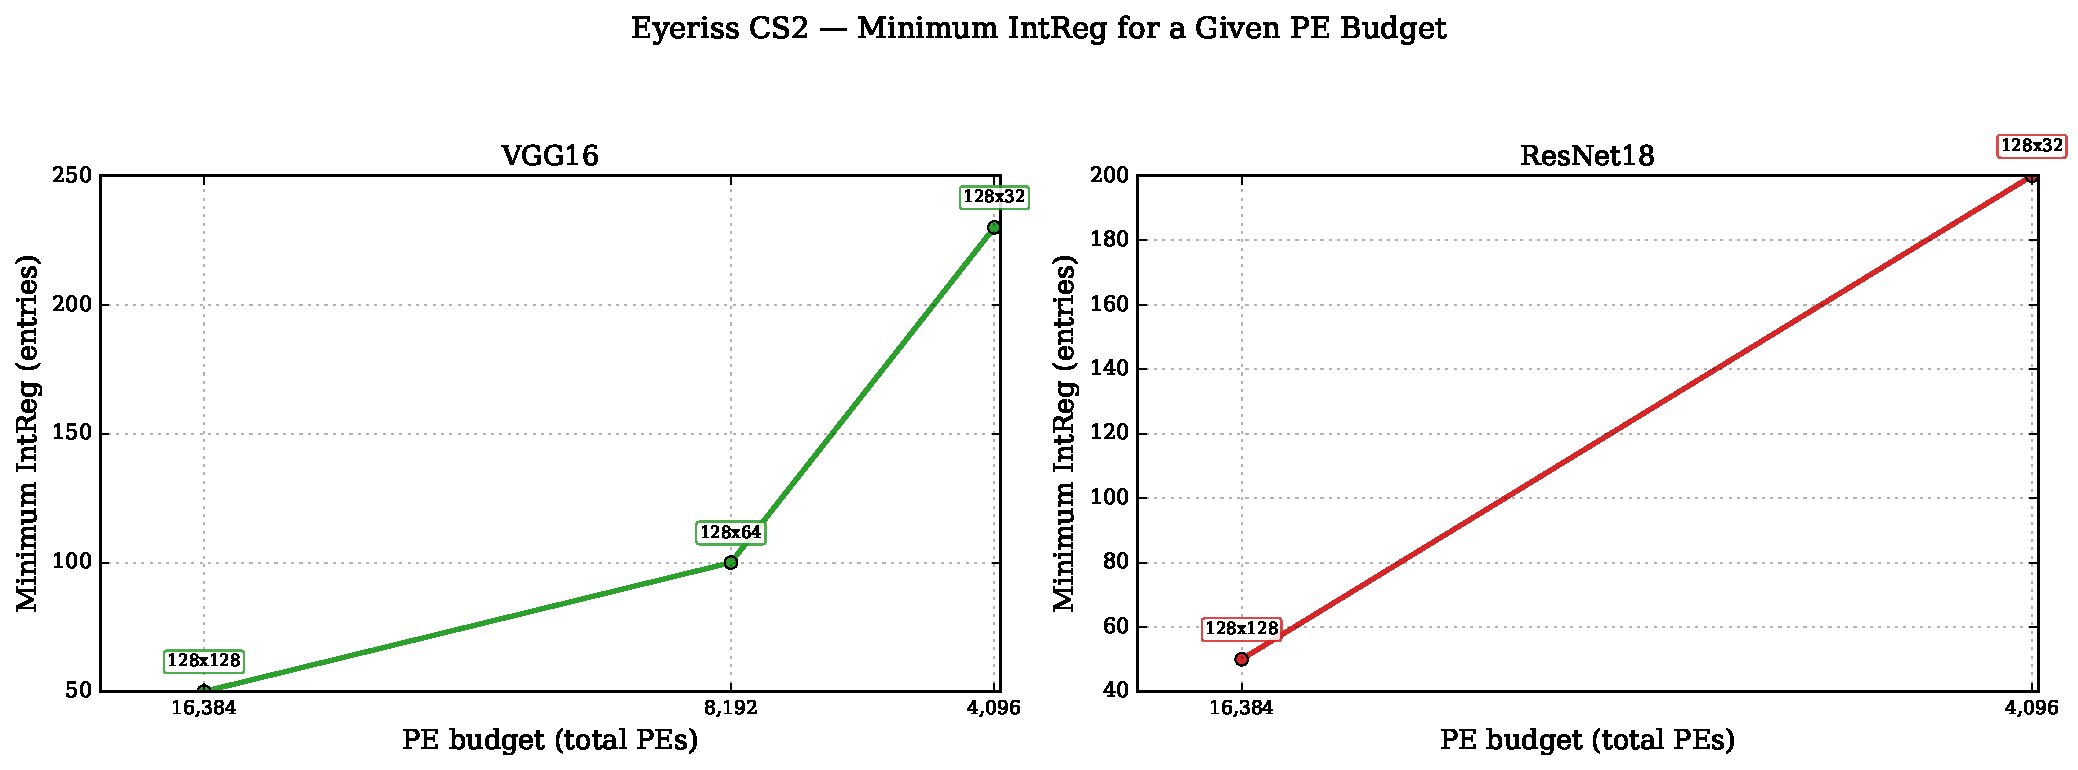
\includegraphics[width=0.85\textwidth]{plots/eyeriss_cs2_intreg_inverted.pdf}
  \caption{Eyeriss CS2: Minimum IntReg required as a function of PE
    budget (VGG16 and ResNet18, full fusion).}
  \label{fig:eyeriss-cs2-inv}
\end{figure}

Figure~\ref{fig:eyeriss-cs2cs3} (top row) shows the energy measured
at the minimum-PE configuration for each IntReg size.
Energy increases monotonically with IntReg, because a larger register
incurs a higher access cost on every read.
For ResNet18 the increase is $1.4\times$ from IntReg\,=\,50 to
IntReg\,=\,1\,000 ($5.15 \times 10^{4} \to 7.12 \times 10^{4}$\,
$\mu$J), a modest penalty compared to the $2.2\times$ energy span
caused by WReg in CS1.

\paragraph{CS2 per Activation-dominant workloads (FSRCNN, MC-CNN).}
For these workloads the intermediate register is not the binding
constraint.
In both cases the intermediate footprint is small (16) because these
networks have few fused layers and narrow channels.

% ────────────────────────────────────────────────────────────────────
\label{sec:eyeriss-cs3}

\paragraph{CS3}
The output register stores only the last fused layer's channel
residual, so its footprint is inherently smaller than that of IntReg
or WReg.
The original single-layer Eyeriss design uses OutReg\,=\,16 entries,
and this value turns out to be sufficient for full fusion as well at
the PE budgets that WReg and IntReg already demand.

Table~\ref{tab:eyeriss-cs3-outreg} confirms this.
For ResNet18, OutReg\,=\,16 requires $128 \times 32 = 4{,}096$~PEs,
which is the saturation point.
The WReg constraint (CS1) already forces 16\,384~PEs at the
tightest feasible point, so
OutReg is therefore automatically satisfied whenever WReg is.
VGG16 tells the same story: OutReg\,=\,16 fits at
$128 \times 32 = 4{,}096$~PEs, which is also the saturation point.

\begin{table}[htbp]
  \centering
  \caption{Eyeriss CS3: Minimum PE count as a function of OutReg
    size (VGG16 and ResNet18, full fusion).
    All other registers are non-binding.}
  \label{tab:eyeriss-cs3-outreg}
  \begin{tabular}{llrrr}
    \toprule
    Workload & OutReg & Config & Total PEs & Saturation \\
    \midrule
    VGG16    &   4 & $128 \times 128$ & 16\,384 & \\
    VGG16    &   8 & $128 \times  64$ &  8\,192 & \\
    VGG16    &  16 & $128 \times  32$ &  4\,096 & $\checkmark$ \\
    \midrule
    ResNet18 &   8 & $128 \times  64$ &  8\,192 & \\
    ResNet18 &  16 & $128 \times  32$ &  4\,096 & $\checkmark$ \\
    \bottomrule
  \end{tabular}
\end{table}

Figure~\ref{fig:eyeriss-cs3-inv} shows the inverted view.
The curves lie well below the corresponding CS1 and CS2 curves at
every PE budget, confirming that OutReg is the least binding of the
three register types.
For activation-dominant workloads (FSRCNN, MC-CNN) the output register
has no effect on the PE count whatsoever: all tested OutReg sizes yield
the same minimum configuration.

\begin{figure}[htbp]
  \centering
  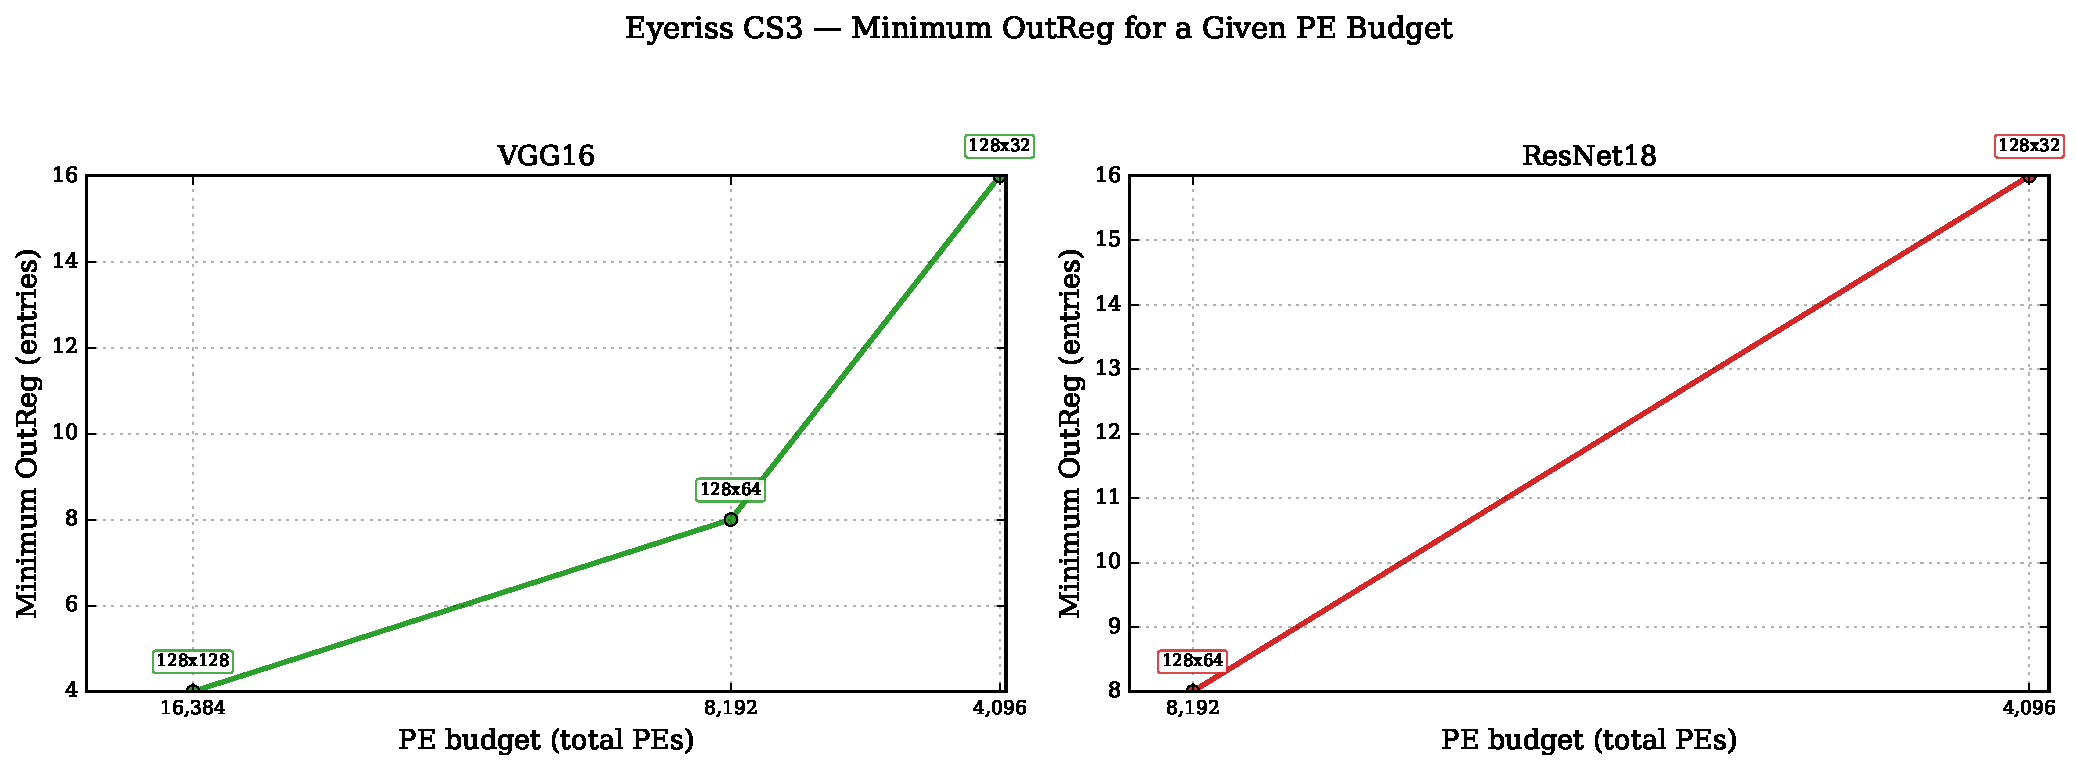
\includegraphics[width=0.85\textwidth]{plots/eyeriss_cs3_outreg_inverted.pdf}
  \caption{Eyeriss CS3: Minimum OutReg required as a function of PE
    budget (VGG16 and ResNet18, full fusion).}
  \label{fig:eyeriss-cs3-inv}
\end{figure}

Analogous reasoning can be applied for Input register sizing.


\paragraph{Considerations}
The intermediate register follows the same PE-doubling-per-halving
rule as the weight register, but its absolute footprint is roughly
one order of magnitude smaller, so it becomes binding only at PE
counts well below the WReg minimum.
The output register is even less constraining: with OutReg\,=\,16
(the value used in the original single-layer Eyeriss), the fused
mapping is already feasible at the PE budgets imposed by WReg.
The input register is unaffected by fusion too, because it
handles only the first layer's input and its footprint remains the
same as in single-layer execution.
